\documentclass[letter,11pt,oneside]{article}
% /home/git/pre/pre.banzai-pipe/tex/BanzaiPipeline.tex
%%% (occur "\\(\\\\[sub]*section\\|appendix\\|input\\|\\<include\\>\\)")
%%% ADDAPPENDIX
%%% APPENDIX
%%% ENDDOC
%%% HEREHEREHERE

\usepackage{color}               %% colored letters {\color{red}{{text}}
\usepackage[listings,breakable]{tcolorbox}
%\usepackage[top=2cm, bottom=2cm, outer=0cm, inner=0cm]{geometry}
\usepackage[pages=some]{background}
\usepackage{fancyhdr}            %% headers/footers
\usepackage{fancyvrb}            %% headers/footersbreakable
\usepackage{datetime}            %% pick up tex date time 
\usepackage{lastpage}            %% support page of ...lastpage
\usepackage{times}               %% native times roman fonts
\usepackage{textcomp}            %% trademark
\usepackage{amssymb,amsmath}     %% greek alphabet
\usepackage{parskip}             %% blank lines between paragraphs, no indent
\usepackage{shortvrb}            %% short verb use for tables
\usepackage{lscape}              %% landscape for tables.
\usepackage{longtable}           %% permit tables to span pages wg-longtable
\usepackage{multicol}            %% Enhance footnotes/endnotes
\usepackage{url}                 %% Make URLs uniform and links in PDFs
%%\usepackage{enumerate}           %% Allow letters/decorations for enumerations
\usepackage{enumitem}           %% Allow letters/decorations for enumerations
\usepackage{endnotes}            %% Enhance footnotes/endnotes
\usepackage{listings}            %% Make URLs uniform and links in PDFs
\pdfadjustspacing=1                %% force LaTeX-like character spacing
%%\usepackage{geometry}            %% allow margins to be relaxed
%%\usepackage{wrapfig}             %% permit wrapping figures.
\usepackage{subfig}              %% images side by side.
%%\geometry{margin=1in}            %% Allow narrower margins etc.
\usepackage[T1]{fontenc}         %% Better Verbatim Font.
\renewcommand*\ttdefault{txtt}   %% 
\usepackage[bookmarks]{hyperref} %% Make huperlinks within a PDF
%%\usepackage{natbib}   %% bibitems
\usepackage{dirtree}


\usepackage{graphicx}            %% Include pictures into a document
%% (wg-texdoc-inserttikz)

%%%%%%%%%%%%%%%%%%%%%%%%%%%%%%%%% PAGE SIZE %%%%%%%%%%%%%%%%%%%%%%%%%%%%%%%%%%%%%%%%%%%%
\pagestyle{fancy}
\usepackage[paperheight=7.125in,paperwidth=9.5in,footskip=.05in,margin=.75in,heightrounded]{geometry}
% (iv (setq tmp (/ (* 3.0 9.5) 4.0 )))   7.125
\fancyhf{}

\def\documentisdraft{NOTDRAFT}

%% (wg-texdoc-isdraft)


\def\drafttest{DRAFT}
\def\wgdocdate{07 Apr, 2020}
\def\wgdocdatetime{\wgdocdate at \currenttime}
\ifx\documentisdraft\drafttest
\usepackage[left]{lineno}   %%%%%%%%%%%%% DRAFT
\usepackage{draftwatermark}
%%\SetWatermarkScale{5.0}
%%\SetWatermarkColor[gray]{0.3}
\fi

%% (wg-texdoc-insert-fancy-headers)

\usepackage[bookmarks]{hyperref} %% Make huperlinks within a PDF
\usepackage{makeidx}             %% Make an index uncomment following line
\makeindex                       %%.. yeah this one, too. index{key} in text
%%



\definecolor{verbcolor}{rgb}{0.6,0,0}
\definecolor{darkgreen}{rgb}{0,0.4,0}
\newcommand\debate[1]{\textcolor{darkgreen}{DEBATE: #1} \marginpar{\textcolor{red}{DEBATE} }}
\newcommand{\ltodo}[2]{\marginpar{\textcolor{red}{ACTION: #1}\endnote{ACTION: #2}}}
\renewcommand{\thefigure}{\thesection-\arabic{figure}}
\newcommand{\menu}{\ensuremath{\;\rightarrow\;}}
\newcommand{\dhl}[1]{{\color{verbcolor}{\texttt#1}}}
\definecolor{wglightgreen}{rgb}{0.88, 0.58, 0.88}
\newcommand{\wgtextbox}[1]{\noindent\fcolorbox{darkgreen}{wglightgreen}{%
    \minipage[t]{\dimexpr0.80\linewidth-2\fboxsep-2\fboxrule\relax}
        {#1}
    \endminipage}}
%%(wg-add-inline-images)  %% add inline images to the mix


%\renewcommand\theendnote{\fnsymbol{endnote}}
\tcbset{colback=green!10!white}


%%Begin User Definitions: Hint: ~/.latex.defs and  latex.defs  
%%End User Definitions:
%%(wg-texdoc-adjust-paper-width)
%% (wg-texdoc-insert-hypersetup)

%%% PDF Fields uncomment \usepackage[bookmarks]{hyperref} above.
\hypersetup{
colorlinks=true,
linkcolor=red,
citecolor=red,
urlcolor=blue,
pdfauthor = {Copyright(c) 2015. All rights reserved. Wayne Green},
pdftitle = {Dainty Ditty's for Astro-Informatic Dockers},
pdfsubject = {Mixing astrometry code.},
pdfkeywords = {Dockerfile, Astronometry.net,sextractor,psfex,python},
pdfcreator = {LaTeX with hyperref package},
pdfproducer = {dvips + ps2pdf}}




%%%%%%%%%%%%%%%%%%%%%%%%%%%%%%%%%%%%%%%%%%%%%%%%%%%%%%%%%%%%%%%%%%%%%%%%%%%%%


\begin{document}


%% (wg-latex-pretty-title-page)
%% (wg-texdoc-titleblock)

\backgroundsetup{
scale=1,
color=black,
opacity=0.7,
angle=0,
contents={%
  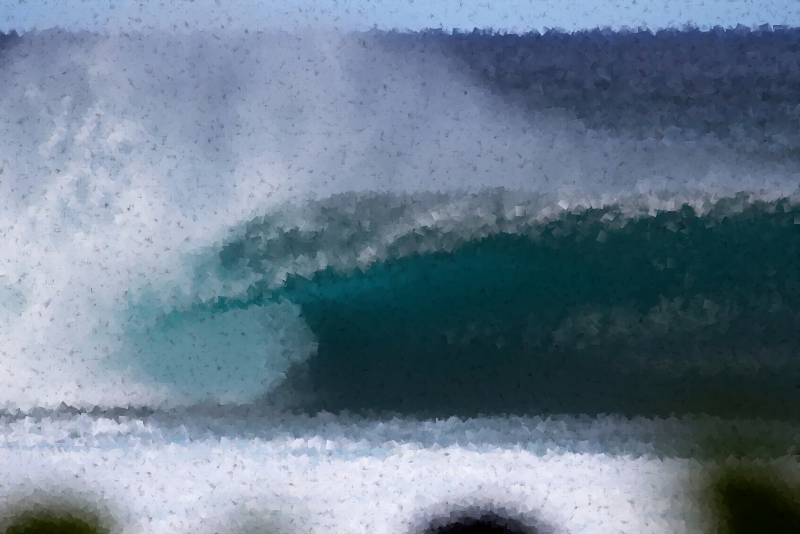
\includegraphics[width=\paperwidth,height=\paperheight]{images/Empty_wave_at_Banzai_Pipeline.png}
  }%
}

\BgThispage
%% \begin{figure}[h!]
%% \centering
%% 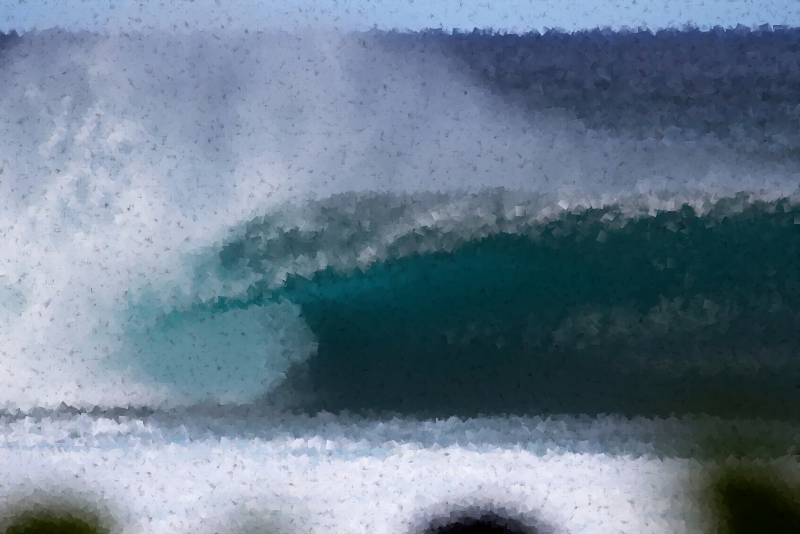
\includegraphics[width=.52\textwidth]{images/Empty_wave_at_Banzai_Pipeline.png}
%% \end{figure}
%% \hskip 9cm {\tiny Apples and Worms and OSs}


\title{\vspace{-1.1cm}
  {\huge \emph{{\color{darkgreen}``Dainty Ditty's for Astro-Informatic Dockers''}}} \\
  {\large Docker Containers} \\
  {\large Astrometry.net} \\
  {\large Sextractor / PSFEx / SCAMP / SWARP} \\
  {\large Astropy and Custom Python} \\
  {\large PostgreSQL and Q3C} \\
  {\large Texlive} \\
  {\large Sphinx} \\
  {\small Local repositories / conda channels / and other containerized tools}}
\author{\vspace{-0.5cm} Wayne Green}
\date{\vspace{-0.5cm} \today}
\maketitle



\pagenumbering{gobble}
\clearpage

% This is tied to certain citations.

\def\wgtrademark{\raise.73ex\hbox{\tiny{\textregistered}}\;}
\def\wgcopyright{\raise.73ex\hbox{\tiny{\copyright}}\;}

\vskip 3cm

\begin{quote}
%%
%%  This document represents my pesonal notes about the landscape
%%  related to deploying science research in and amoung my
%%  colleagues. It is freely available, and worth every penny! While I
%%  retain copyright, this is soley to prevent its mis-appropriation for
%%  others' private or commercial uses. While an effort was made to
%%  cite every product etc some will have been missed.  This information
%%  and code snippets are provided, as is,  under the MIT license for others.
%%  
{ Copyrights and Trademarks:\\ 
\\
Arduino 2022, under Creative Commons licensing;
Anaconda is a collection of Python and analytic tools by Anaconda\wgtrademark Inc.;
Apple\wgtrademark, iOS\wgtrademark,
  OS/X\wgtrademark and Macbook\wgtrademark are a trademarks of Apple Inc., registered 
in the U.S. and other countries;
   Astrometry.net Copyright 2006-2010 Michael Blanton, David W. Hogg, Dustin Lang, 
Keir Mierle and Sam Roweis, Copyright 2011-2013 Dustin Lang and David W. Hogg. 
Copyright 2006-2022 Michael Blanton, David W. Hogg, Dustin Lang, Keir Mierle and 
Sam Roweis \cite{arXiv:0910.2233} (the Astrometry.net Team);
   The Astropy Project \cite{astropy:2018} is a loose-confederation funded by NumFOCUS, Inc.;
Docker, Inc. provides the technology for Docker Environments, Containers etc, \textcopyright 2013-2015 Docker, Inc. All rights reserved;
IRAF, PyRAF and Ureka Copyright \textcopyright 2018 Association of Universities for Research in
  Astronomy (AURA);
  Bokeh,2021 Bokeh Contributors,  is a fiscally sponsored project of NumFOCUS;
  Django The Django Software Foundation;
  NumPy   \textcopyright 2005-2018, NumPy Developers ;
  The ``Math Kernel Library'' (MKL\wgtrademark) and Intel\wgtrademark are registered
  by Intel Corporation -- Santa Clara, CA, USA;
Microsoft, ``Microsoft Windows'', WSL are registered trademark of Microsoft Corporation;
PostgreSQL\wgtrademark is a registered trademark of 
   PostgreSQL Global Development Group;
Python is Copyright \textcopyright 2001-2018 Python  Software Foundation.
   All rights reserved ;
Raspberry Pi, governed by the Raspberry Pi Foundation with offerings covered by the
Creative Commons CC BY-SA licensing;
SAOImage/ds9 and code therein is licensed through the 
   Smithsonian Astrophysical Observatory;
SExtractor \cite{web-sextractor} (Emmanuel Bertin, author) copyright
   \textcopyright 2010 IAP - CNRS / Universite P.\&M.Curie ;
Ubuntu \textcopyright 2015 Canonical Ltd. Ubuntu and Canonical are registered 
  trademarks of Canonical  Ltd;
UNIX\wgtrademark is a registered trademark in
  the United States and other countries, licensed exclusively through
  X/Open Company Ltd;
  Linux\wgtrademark is the registered trademark of Linux Mark Institute,
  on behalf of Linus Torvalds, in the U.S. and other countries.
  \\
  ~
}



\end{quote}
{\tiny
Copyright \wgcopyright (2020) Wayne Green. All rights reserved.

Permission is hereby granted, free of charge, to any person obtaining
a copy of this software and associated documentation files (the
"Software"), to deal in the Software without restriction, including
without limitation the rights to use, copy, modify, merge, publish,
distribute, sublicense, and/or sell copies of the Software, and to
permit persons to whom the Software is furnished to do so, subject to
the following conditions:

The above copyright notice and this permission notice shall be
included in all copies or substantial portions of the Software.

THE SOFTWARE IS PROVIDED "AS IS", WITHOUT WARRANTY OF ANY KIND,
EXPRESS OR IMPLIED, INCLUDING BUT NOT LIMITED TO THE WARRANTIES OF
MERCHANTABILITY, FITNESS FOR A PARTICULAR PURPOSE AND
NONINFRINGEMENT. IN NO EVENT SHALL THE AUTHORS OR COPYRIGHT HOLDERS BE
LIABLE FOR ANY CLAIM, DAMAGES OR OTHER LIABILITY, WHETHER IN AN ACTION
OF CONTRACT, TORT OR OTHERWISE, ARISING FROM, OUT OF OR IN CONNECTION
WITH THE SOFTWARE OR THE USE OR OTHER DEALINGS IN THE SOFTWARE.
}

\pagenumbering{gobble}
\clearpage


%%%%%%%%%%%%%%%%%%%%%%%%%%%%%%%%%%%%%%%%%%%%%%%%%%%%%%%%%%%%%%%%%%%%%%%%%%%%%
%% table of contents
%%%%%%%%%%%%%%%%%%%%%%%%%%%%%%%%%%%%%%%%%%%%%%%%%%%%%%%%%%%%%%%%%%%%%%%%%%%%%
 

%%\pagenumbering{gobble}   %ignore page numbers for a while
\pdfbookmark[0]{Table of Contents}{MyTOC} % if usepackage{hyperref} in use.
\begin{multicols}{2}
  \tableofcontents
\end{multicols}

\listoffigures
%\listoftables
\clearpage
\cfoot{{\tiny Page \thepage \hspace{1pt}}}
\pagenumbering{roman}   % i,ii,etc

\section*{Preface}

This document contains notes about building a photometry pipeline in
a docker environment for Linux and Win10.

First and foremost ``Docker Containers'' (containers) are ``designed''
for developers, used for ``service deployment'' and (while desirable),
not for ``application deployment''.

In the context of this article, a certain vocabulary is created to
help avoid confusion -- especially with overloaded terms:

\dhl{PMachine} - the Physical machine you can touch, that holds logical
containers. The OS is usually referred to as the \dhl{host} os.

\dhl{CMachine} - a 'Container' with its view of a 'OS'. In short most
of the time CMachines think they are PMachines -- same commands,
same network issues, etc.

\dhl{X11} - The mainstay of the Unix windowing system that consists
of 1) \dhl{clients} -- programs creating output for display, buttons
to push, image frames to show graphs etc and 2) \dhl{servers} -- the
logic that accepts those commands and actually ``renders the content''
to a 'screen'. The sense of CLIENT and SERVER is backwards to that of
a database. X11 is old, robust, made to support graphics in the times
of dial-up modems and is very light-weight in its bandwidth overhead.
It is NOT your great-grandson's Wayland \index{Wayland} -- while
still pending for Ubuntu 20.04, support is still weak.

Docker extends the host's hardware which is simply a ``Physical
Machine'' (\dhl{PMachine}) with modern hyper-visor support.

A PMachine runs a container that ``believes'' it is a physical
machine.  A container, herein, is refereed to as a ``Container Machine''
(\dhl{CMachine}). Remember, PMachines have atoms and CMachines have
electrons. A container is managed by a daemon that uses hypervisor
functionality to 'glue' the OS within the container (CMachine) to its
'host' (PMachine).

A container is an empty light-weight hypervisor interface that is
filled first with a Linux based OS then filled with any user code.


\begin{tcolorbox}
\begingroup \fontsize{10pt}{10pt}
\selectfont
%%\begin{Verbatim} [commandchars=\\\{\}]
\begin{verbatim} 
here:me> docker export <CONTAINER ID> > /home/export.tar
here:me> scp /home/export.tar them@there.net:/home/them
there:them> cat /home/export.tar | docker import - some-name:latest
\end{verbatim}
\endgroup
%% \end{Verbatim}
\end{tcolorbox}


The argument over who owns the PMachine's GUI user experience becomes,
well, quite territorial when it comes to hosting mainstay X-Windows
environment in a Microsoft OS or in Apple iOS's diverging OS. You may
be better served with a VBox\footnote{Oracle Corp. VirtualBox or other
vendors equivalents.}. Each camp can make a compelling argument
to the user while avoiding the user's real need -- to express their
problem to software while the 'interface' is invisible. To take the
user's focus away from their problem is, well not a Good
Thing(\texttrademark).

The learning curve for this task is as straight-forward as stepping of
a high cliff.  Today, \today, a decent task it to encapsulate a body
of 'codes'\footnote{I'm an astronomer with a storied career in
  computing.} that are critical to science and somewhat lost to
history.

\ltodo{Flesh out hypevisors}{The origin of a 'hypervisor' is hard to nail down but
today it is usually interpreted to mean running one OS within
another.}

\clearpage

\setcounter{section}{0}
\pagenumbering{arabic}


\section{Important Details}

These notes are from a Linux perspective. 

When you use the container, it's transient (current) state will not
``persist''; therefore any newly created files inside its file system
are lost. THE STATE IS LOST WHEN THE CONTAINER STOPS!  That is a Good
Thing(\texttrademark)... you always start fresh.

You can ``pause'' and ``commit'' the running container with a new
tag/version. Pick up where you leave off. This is handy as checkpoints
for containers running in production -- where one may restore to
a recent/earlier state. 

Cast of characters: the \dhl{\$USER} is Bob Brown (herein bob),
with  \dhl{/home/bob} as the \dhl{\$HOME} directory.


\ltodo{perspective}{The container is built using the
  \dhl{continuum/anaconda} container using a reasonably current core
  Ubuntu 18.04 OS. The ``Dockerfile'' for the container is in Appendix
  \ref{sec:Dockerfile}. Remember, Ubuntu 18.04 still supports 32-bit
  libraries.}


\clearpage

There are massive confusions surrounding the terms ``host'',
``client'' and ``server''. These are overloaded terms. Again, for
clarity, the term \dhl{PMachine} will refer to the physical machine
controlling your Desktop, and the term \dhl{CMachine} represents the<>
``containerized'' machine. \index{PMachine!ref} \index{CMachine!ref}
\index{PMachine!server} \index{PMachine!client''}
\index{PMachine!host''} \index{CMachine!server}
\index{CMachine!client''} \index{CMachine!host''}

\begin{figure}[h!]
\centering
\subfloat[X11]{{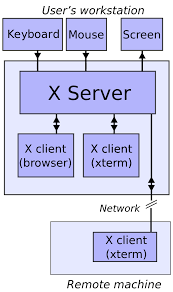
\includegraphics[width=.25\textwidth]{images/Xwindows.png}}}%
\qquad
\subfloat[Wayland]{{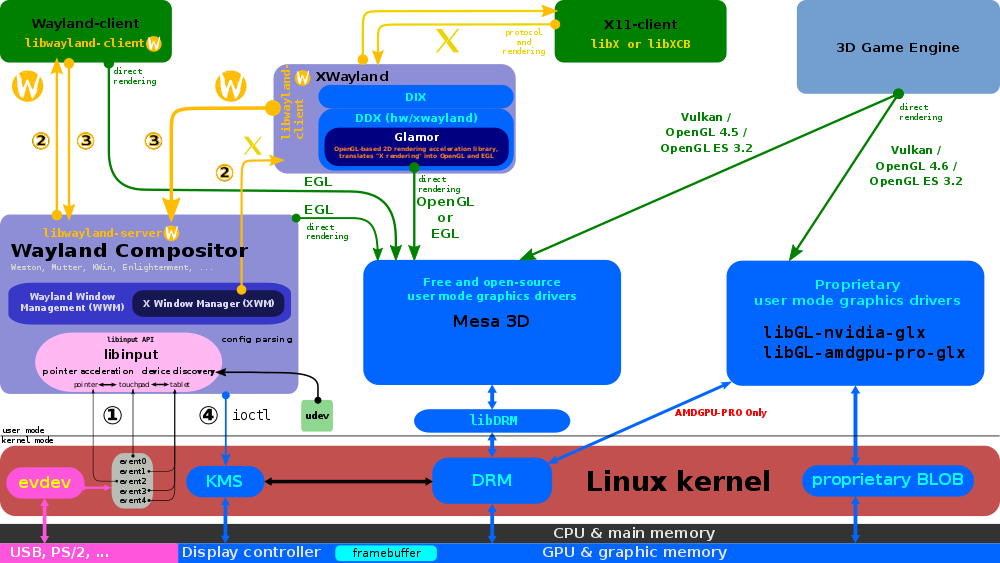
\includegraphics[width=.65\textwidth]{images/1000px-The_Linux_Graphics_Stack_and_glamor.png}}}%
\caption[X11 vs Wayland]{The reversed sense of 'server' and client' in X-Windows.\\
  {\tiny{(a) David Gerard ~ ~ (b) \url{https://commons.wikimedia.org/wiki/User:ScotXW}}}} 
\label{figure:ServerClient}
\end{figure}


W.r.t. X11, the term ``server'' is the OS's GIO window that ``serves''
the information from a program (X ``client'') to your eyeballs. The
``client'' does the heavy-lifting/computations to producing the
text/images. In normal computing the term ``Server'' refers to the
program/hardware doing the computations and producing the text/images
and the ``Client'' some task or person utilizing the service.

Unix OSs perceive themselves to be ``peers'', so the whole
Host/Client thing is relative.

The user-level ``Docker Desktop'' has to be installed on your PMachine:
\index{docker!desktop}

\url{https://www.docker.com/get-started}

On your PMachine: Create a directory called \dhl{\$HOME/Astro}.

Under this directory you should put everything containers need
access. This is all the fits files, etc. It is the ``link'' between
the CMachine and that part of your PMachine.


A few additional key files are supplied:

%% \begin{tcolorbox}
%% \begingroup \fontsize{10pt}{10pt}
%% \selectfont
%% %%\begin{Verbatim} [commandchars=\\\{\}]
%% \begin{verbatim} 
%% iraf.aliases      (handy bash aliases)
%% Aluminum.keycodes (if you need them)
%% Xmodmap           (for oddball keyboards)
%% \end{verbatim}
%% \endgroup
%% %% \end{Verbatim}
%% \end{tcolorbox}

\ltodo{Additional Software}{Any mass of things needed by one or
more contaienrs.}

A few critical aliases:

%% \begin{tcolorbox}
%% \begingroup \fontsize{10pt}{10pt}
%% \selectfont
%% %%\begin{Verbatim} [commandchars=\\\{\}]
%% \begin{verbatim} 
%% alias iraf27="source activate iraf27"
%% alias pyraf="(export PYTHONSTARTUP=$HOME/iraf/pyraflogin.py; \
%%     /opt/conda/envs/astrocondairaf/bin/pyraf -s; )"
%% \end{verbatim}
%% \endgroup
%% %% \end{Verbatim}
%% \end{tcolorbox}
%% 
%% The program \dhl{pyraflogin.py} (see
%% \cite{PyrafProgrammersGuide,CLProgrammersGuide}) is an exercise in
%% extending the pythonic wrapper for PyRAF. Based on the literature and
%% some hacking the ability to make matplotlib graphs, and to save
%% intermediate results etc are promoted.  \index{PyRAF!pyraflogin}
%% \index{pyraflogin!PyRAF}
%% 
%% The git repository:
%% 
%% \url{https://github.com/dxwayne/Banzai-Pipeline}
%% 
%% ...may be \dhl{git cloned} into the \dhl{\$home/astro/iraf}
%% directory. It winds up below the normal \dhl{iraf} directory contents
%% and is essentially invisible to PyRAF/IRAF. However, you may copy
%% some of its contents up into \dhl{\$HOME/iraf} as you like.


\clearpage


\ifx\documentisdraft\drafttest
\linenumbers    %%%%%%%%%%%%% DRAFT
\fi

\section{Astrometry.net}

Github has a working image of the file.


\section{Networking}

Astronomy applications use SAMP and XPA.
Programs like the Virtual Observatory (VO) \cite{1998AAS...192.6401D},
Aladin \cite{2000A&AS..143...33B},
SAOImage/ds9 \cite{2003ASPC..295..489J},
TOPCAT/ADQL \cite{2005ASPC..347...29T,2017ASPC..512..589T},
SPLAT-VO \cite{2014A&C.....7..108S} readily inter-operate with
PMachine/CMachine databases like PostgreSQL. This requires
careful management of TCP/IP Port access, the docker bridge
and the local PMachine IPTables, etc.

Docker runs containers within a \dhl{docker bridge} -- this requires
some fancy dancing to get a connection between the PMachine and a
CMachine. \index{docker!bridge}

\begin{tcolorbox}
\begingroup \fontsize{10pt}{10pt}
\selectfont
%%\begin{Verbatim} [commandchars=\\\{\}]
\begin{verbatim} 
https://docs.docker.com/engine/reference/commandline/attach/
https://runnable.com/docker/basic-docker-networking

# good youtubes on networking
https://www.youtube.com/watch?v=Yr6-2ddhLVo
https://cntnr.io/running-guis-with-docker-on-mac-os-x-a14df6a76efc  ***
\end{verbatim}
\endgroup
%% \end{Verbatim}
\end{tcolorbox}




%%% APPENDIX
\appendix
\renewcommand \thesection{\Alph{section}}

\section{Overview}

Docker ``Containers'' contain, initialize and run a Docker ``Image''.

A Docker images is built from a ``Dockerfile'' using \dhl{docker build ...}.

A ``Container'' can be created from a ``Image'' using \dhl{docker create ...}.
\clearpage


\dirtree{%
.1 Observations.
.2 \dhl{/ddMMMyyyy/}  \# \dhl{local dates data}.
.3 usw                \# \dhl{Nights collection}.
.4 reduce.cl          \# \dhl{template}.
.4 reduce.pyraf       \# \dhl{template}.
.3 RawData            \# \dhl{Nights Raw Data}.
.3 PreAnalysis        \# \dhl{The basic work}.
.3 Analysis           \# \dhl{Non-pipeline work for pre-publication}.
.2 usw                \# \dhl{Global templates etc}.
.3 Targets            \# \dhl{Global target collection usws}.
.4 \dhl{<target>}.
.5 hints.ans.
.5 cfg.ans.
.5 target.tsv.
.5 finder.png.
.5 Catalog\_AAVSO.tsv.
.5 Catalog\_UCAC4.tsv.
.5 Catalog\_REFCAT2.tsv.
}


Layout of the the Observations Environment. The collection of all the
observations, general aspects of a user's environment like ds9 fiture
templates etc; each target (defining the location and header details),
each night observations -- their rawdata, preanalysis (augmenting
headers, bias/dark/flats, specific reduce.cl; etc), and any analysis
prior to publication. Should be under revision management.

\clearpage


\section{Deployment}

The first container to make is the \dhl{Dockerfile.xeyes} container
test on the local PMachine that supports X11, then

\begin{tcolorbox} %[breakable,colback=yellow!5!black]
\begingroup \fontsize{10pt}{10pt}
\selectfont
%%\begin{Verbatim} [commandchars=\\\{\}]
\begin{verbatim} 
docker run -v /tmp/.X11-unix:/tmp/.X11-unix  \
  -e DISPLAY=$DISPLAY  \
  -h $HOSTNAME  \
  -v $HOME/.Xauthority:/home/lyonn/.Xauthority  \
  --name xeyestest \
  ubuntu_xeyes:1
\end{verbatim}
\endgroup
%% \end{Verbatim}
\end{tcolorbox}

while it is running:

\begin{tcolorbox} %[breakable,colback=yellow!5!black]
\begingroup \fontsize{10pt}{10pt}
\selectfont
%%\begin{Verbatim} [commandchars=\\\{\}]
\begin{verbatim} 
docker export xeyestest | gzip > ubuntu_xeyes_1.tar.gz
\end{verbatim}
\endgroup
%% \end{Verbatim}
\end{tcolorbox}

The \dhl{ubuntu\_xeyes\_1.tar.gz} file is then copied to the 'other'
PMachine. For Win10

% HEREHEREHERE

\section{Docker Security}

Docker interactions are centered around a daemon \dhl{dockerd}
\footnote{\url{https://docs.docker.com/engine/reference/commandline/dockerd/}}.

Docker relies heavily on Unix Namespaces, its own TCP/IP stack and
bridge arrangements, Unix sockets, and the TCP/IP stack of the machine
to facilitate communications between the PMachine and the CMachine via
the docker daemon. This should be restricted to local host
\dhl{127.0.0.1}. By default it uses port \dhl{2345} for insecure
transactions and port \dhl{2346} for secure transactions.  Other
tricks using Certificates of Authority (CA) etc help to further
isolate PMachine/CMachine interface and CMachine/CMachine
interoperability. \index{docker!security}

Starting services: systemd vs systemV -- Ubuntu uses systemd, alpine
uses systemV.

\ltodo{flesh out systemd}{Get a crib together for this.}


\url{https://towardsdatascience.com/analyzing-docker-image-security-ed5cf7e93751}\
\section{X11}

\begin{tcolorbox} %[breakable,colback=yellow!5!black]
\begingroup \fontsize{10pt}{10pt}
\selectfont
%%\begin{Verbatim} [commandchars=\\\{\}]
\begin{verbatim} 
PMachine needs ``X11FORWARDING yes'' is \dhl{/etc/ssh\_config}
Assure \dhl{/etc/ssh_config}:
X11Forwarding yes
X11DisplayOffset 10
X11UseLocalhost no
sudo service ssh restart
\end{verbatim}
\endgroup
%% \end{Verbatim}
\end{tcolorbox}

\url{https://askubuntu.com/questions/61690/ssh-x-xt-error-cant-open-display-0-0}
supplies obscure background config sources.

Where \dhl{DISPLAY=0} or \dhl{DISPLAY=0.0} means the 'current' window
of a set of virtual/physical displays is in use.  Make sure DISPLAY is
not being set in \dhl{/etc/environment} or \dhl{/etc/bash.bashrc}, or
\dhl{~/.bash.rc} or any \dhl{alias} files it may ingest. Run
\dhl{env | grep DISPLAY}

The command \dhl{ssh -X user@machine env} will show ``environment''
things there.





\section{Local Docker Development Machine}

If on a slow network, then create local repo.

\index{conda!Slow Network}

\begin{tcolorbox}
\begingroup \fontsize{10pt}{10pt}
\selectfont
%%\begin{Verbatim} [commandchars=\\\{\}]
\begin{verbatim} 
apt-get install dpkg-dev
cd /opt
mdkir -p /opt/debrepo  # our local depo
cd /opt/debrepo
cp -p /var/cache/apt/archives/*deb .  # get the packages on HOST here.
dpkg-scanpackages . /dev/null | gzip -9c > Packages.gz
\end{verbatim}
\endgroup
%% \end{Verbatim}
\end{tcolorbox}

\section{PyRAF}

PyRAF within a docker container wants to interact with many support
programs via XPA and SAMP. \index{XPA!PyRAF} \index{SAMP!PyRAF}
\index{PyRAF!XPA} \index{PyRAF!SAMP}


Currently the SAMP and 'message of the day' parts of login.cl
don't allow PyRAF to run. Comment them out.\index{PyRAF!SAMP!login.cl motd}

\section{SAOImage/ds9}

SAOImage/ds9 is an enhanced replacement for the old IRAF ximtool --
itself a replacement for IRAF' tv/display. It implements XPA (Section
\ref{sec:XPA}). Tcl, and toolkit Tk is a dynamic, late-binding (ie
self-modifying) language that, while 'born of frustration' is
frustrating to use owing to a few missed tricks, complicated syntax
and complicated approach to introspection. That said, users' may
extend ds9 in wondrous ways. \index{tcl/Tk overview}.


\section{SAMP}

SAMP runs on port 21012. \dhl{https://localhost:21012} is there! \index{SAMP:port addr}
\cite{SAMP-1,2012ivoa.spec.1104T}. The snippet in Figure \ref{figure:SAMP-Example}
outlines a quick use of Linux utilities to find the host for the hub. It
implements a Unix socket connection using traditional XML-RPC tricks.

\begin{figure}[h!]
  \begin{tcolorbox}
\begingroup \fontsize{10pt}{10pt}
\selectfont
%%\begin{Verbatim} [commandchars=\\\{\}]
\begin{verbatim} 
sudo netstat -lp | grep 21012
tcp6       0      0 [::]:21012    [::]:*   LISTEN      15583/java          

ps aux | grep 15583
wayne    15583  0.7  2.0 13649168 686824 pts/1 Sl...
... Apr02 155:01 java -Duk.ac.starlink.topcat.cmdname=topcat...
... -classpath ./../lib/topcat/topcat.jar:/home/wayne/Configuration//postgresql- ...
... 42.2.8.jar uk.ac.starlink.topcat.Driver
\end{verbatim}
\endgroup
%% \end{Verbatim}
  \end{tcolorbox}
\caption[SAMP Example]{SAMP - Example to find the app listening on port 15583.} 
\label{figure:SAMP-Example}
\end{figure}


\ltodo{Box figure text}{Add a way to make verbatim figures stand out.}

\section{XPA}

XPA like SAMP is a suite of interprocess communications tools. You can
obtain the source code from \url{https://github.com/ericmandel/xpa.git},
or install with the apt-get xpa-tools (and other language dependent libraries).
The GitHub repository has some interesting python tricks. XPA has ties
to tcl making and is the underpinning of the communications between
IRAF/PyRAF and ds9. 
\index{XPA!overview}
\index{ds9!XPA} \index{IRAF/PyRAF!XPA}  \index{XPA!IRAF/PyRAF}
\index{XPA!tcl}

\ltodo{Make XPA docker exercise}{An excellent way to grab a package
  and see what it brings along with it without changing PMachine host.}

\begin{tcolorbox}
\begingroup \fontsize{10pt}{10pt}
\selectfont
%%\begin{Verbatim} [commandchars=\\\{\}]
\begin{verbatim} 
me> xpaget xpans
XPA$ERROR no 'xpaget' access points match template: xpans
me >ds9 &
xpaget xpans
DS9 ds9 gs 7f000001:42049 me
\end{verbatim}
\endgroup
%% \end{Verbatim}
\end{tcolorbox}

The port/server/connections were established when ds9 started:
\dhl{7f000001} string is 127.0.0.1 or localhost is 42049 and the
'user' is me is the port that was established when ds9 started.

XPA has a simple command-line vocabulary that enables a script
(bash/python) to make simple queries in both directions.  Examples for
ds9, while in tcl can be easily transliterated to bash, are at:
\url{http://ds9.si.edu/doc/ref/xpa.html} \index{ds9!XPA!examples}.


DS9 ds9 gs 7f000001:42049 me
\section{bash}

Debian uses a nasty /bin/dash in lieu of bash.
So, \index{bash!dash}

\begin{tcolorbox}
\begingroup \fontsize{10pt}{10pt}
\selectfont
%%\begin{Verbatim} [commandchars=\\\{\}]
\begin{verbatim} 
mv /bin/sh /bin/dashsh
ln -s /bin/bash /bin/sh 
\end{verbatim}
\endgroup
%% \end{Verbatim}
\end{tcolorbox}


A clean \dhl{continuumio/anaconda3} was downloaded, and the packages copied
from the container. This is a rather large directory.

The recipe for IRAF was run:

\begin{tcolorbox}
  \begingroup \fontsize{10pt}{10pt}
\selectfont
%%\begin{Verbatim} [commandchars=\\\{\}]
\begin{verbatim} 
conda create -n iraf27 python=2.7 iraf-all pyraf-all stsci
conda install -c conda-forge jupyter_contrib_nbextensions
\end{verbatim}
\endgroup
%% \end{Verbatim}
\end{tcolorbox}

... and the resulting packages copied.

A small python script:

\begin{tcolorbox}
  \begingroup \fontsize{10pt}{10pt}
\selectfont
%%\begin{Verbatim} [commandchars=\\\{\}]
\begin{verbatim} 
from collections import OrderedDict()
d = OrderedDict()
f = open('pre','r')
x = open('post','r')
for c in f:
   if(c not in d):
      d[c] = []
   d[c].append('pre  '+c.strip())

for c in x:
   if(c not in d):
      d[c] = []
   d[c].append('post '+c.strip())

with open("postpackges.txt",'w') as o:
   for k,v in d.items():
      if(len(v) == 1):
         print("{}".format(v[0]),file=o)
\end{verbatim}
\endgroup
%% \end{Verbatim}
\end{tcolorbox}

A list of places where there was only 1 entry was
created. These were all 'post' by the logic above.

\begin{tcolorbox}
  \begingroup \fontsize{10pt}{10pt}
\selectfont
%%\begin{Verbatim} [commandchars=\\\{\}]
\begin{verbatim} 
cd post
mkdir local-channel
cd local-channel
mkdir linux-64 osx-64
cd linux
cp ../../*.bz2 .
conda index .
#check Note: the two slashes with the file, and --offiline
conda search  --offline -c file://home/wayne/play/bob/oc/gaoiraf iraf-x11 | grep gaoiraf

docker run -it -v /home/wayne/play/bob/oc/gaoiraf:/opt/gaoiraf continuumio/cuupdated
conda config --add channels file://opt/gaoiraf
conda create -c gaoiraf -n iraf27 python=2.7 iraf-all pyraf-all stsci
\end{verbatim}
\endgroup
%% \end{Verbatim}
\end{tcolorbox}

\section{Ubuntu Packages}

Using \dhl{docker pull ubuntu18.04:latest}, build a basic container,
adding a few packages. The file \dhl{/etc/apt/apt.conf.d} contains
several 'rules' for apt to follow.

For the basic container:

\begin{tcolorbox}[breakable]
  % /home/git/pre/DaintyDittys.pre/doc/offlineplay.tex


\begingroup \fontsize{8pt}{8pt}
\selectfont

%%\begin{Verbatim} [commandchars=\\\{\}]
\begin{verbatim} 

### 01-vendor-ubuntu
Acquire::Changelogs::AlwaysOnline "true";
### 01autoremove
APT
{
  NeverAutoRemove
  {
	"^firmware-linux.*";
	"^linux-firmware$";
	"^linux-image-[a-z0-9]*$";
	"^linux-image-[a-z0-9]*-[a-z0-9]*$";
  };

  VersionedKernelPackages
  {
	# linux kernels
	"linux-image";
	"linux-headers";
	"linux-image-extra";
	"linux-modules";
	"linux-modules-extra";
	"linux-signed-image";
	"linux-image-unsigned";
	# kfreebsd kernels
	"kfreebsd-image";
	"kfreebsd-headers";
	# hurd kernels
	"gnumach-image";
	# (out-of-tree) modules
	".*-modules";
	".*-kernel";
	"linux-backports-modules-.*";
	"linux-modules-.*";
        # tools
        "linux-tools";
        "linux-cloud-tools";
	# build info
	"linux-buildinfo";
	# source code
	"linux-source";
  };

  Never-MarkAuto-Sections
  {
	"metapackages";
	"contrib/metapackages";
	"non-free/metapackages";
	"restricted/metapackages";
	"universe/metapackages";
	"multiverse/metapackages";
  };

  Move-Autobit-Sections
  {
	"oldlibs";
	"contrib/oldlibs";
	"non-free/oldlibs";
	"restricted/oldlibs";
	"universe/oldlibs";
	"multiverse/oldlibs";
  };
};
### 01autoremove-kernels
// DO NOT EDIT! File autogenerated by /etc/kernel/postinst.d/apt-auto-removal
APT::NeverAutoRemove
{
   "^linux-image-4\.4\.0-174-generic$";
   "^linux-headers-4\.4\.0-174-generic$";
   "^linux-image-extra-4\.4\.0-174-generic$";
   "^linux-modules-4\.4\.0-174-generic$";
   "^linux-modules-extra-4\.4\.0-174-generic$";
   "^linux-signed-image-4\.4\.0-174-generic$";
   "^kfreebsd-image-4\.4\.0-174-generic$";
   "^kfreebsd-headers-4\.4\.0-174-generic$";
   "^gnumach-image-4\.4\.0-174-generic$";
   "^.*-modules-4\.4\.0-174-generic$";
   "^.*-kernel-4\.4\.0-174-generic$";
   "^linux-backports-modules-.*-4\.4\.0-174-generic$";
   "^linux-modules-.*-4\.4\.0-174-generic$";
   "^linux-tools-4\.4\.0-174-generic$";
   "^linux-cloud-tools-4\.4\.0-174-generic$";
};
/* Debug information:
# dpkg list:
# list of installed kernel packages:

# list of different kernel versions:

# Installing kernel:  ()
# Running kernel: ignored (4.4.0-174-generic)
# Last kernel: 
# Previous kernel: 
# Kernel versions list to keep:

# Kernel packages (version part) to protect:
4\.4\.0-174-generic
*/
### 70debconf
// Pre-configure all packages with debconf before they are installed.
// If you don't like it, comment it out.
DPkg::Pre-Install-Pkgs {"/usr/sbin/dpkg-preconfigure --apt || true";};
### docker-autoremove-suggests
Apt::AutoRemove::SuggestsImportant "false";
### docker-clean
DPkg::Post-Invoke { "rm -f /var/cache/apt/archives/*.deb /var/cache/apt/archives/partial/*.deb /var/cache/apt/*.bin || true"; };
APT::Update::Post-Invoke { "rm -f /var/cache/apt/archives/*.deb /var/cache/apt/archives/partial/*.deb /var/cache/apt/*.bin || true"; };
Dir::Cache::pkgcache ""; Dir::Cache::srcpkgcache "";
### docker-gzip-indexes
Acquire::GzipIndexes "true"; Acquire::CompressionTypes::Order:: "gz";
### docker-no-languages
Acquire::Languages "none";
\end{verbatim}
\endgroup
%% \end{Verbatim}

\end{tcolorbox}

Packages consists of a \dhl{Package.gz} file made with:

\dhl{apt-get download <packages...>} they wind up in the directory
/var/cache/apt/archives

\dhl{dpkg-scanpackages . /dev/null | gzip -9c > Packages.gz}

/etc/apt/apt.conf.d

\section{The Anaconda Part}

Anaconda downloads and retains the individual packages in
/opt/conda/pkgs

A run of the Dockerfile, with a log of the results was made and
retained.



\begin{tcolorbox}
  \begingroup \fontsize{10pt}{10pt}
\selectfont
%%\begin{Verbatim} [commandchars=\\\{\}]
\begin{verbatim} 
docker pull continuumio/anaconda3
docker exec -it continuumio/anaconda3 /bin/bash
conda update
apt-get install -y vim
# set up for 32-bit libraries, update aptitude
dpkg --add-architecture i386
apt-get update
apt-get install -y libstdc++6:i386

apt-get install -y xorg  # add in the X11 stuff.
QUESTION ABOUT KEYBOARD!!!
apt-get install -y --reinstall procps
apt-get install -y net-tools             # ifconfig
apt install -y iproute2                  # ip in leiu of ifconfig
apt-get install -y rsyslog               # some decent logging
apt-get install -y openssh-server        # ssh into the container


...
# in the HOST window!
docker ps -a                                 # get xxxxxxxx id for container.
docker stop xxxxxxxx
docker commit xxxxxxxx continuumio/c3updated # save investment at this point.
docker exec -it continuumio/c3updated /bin/bash


# Back to the new container

conda config --add channels http://ssb.stsci.edu/astroconda
conda create -n iraf27 python=2.7 iraf-all pyraf-all stsci
conda install -c conda-forge jupyter_contrib_nbextensions
useradd -m -d /home/bob -G dialout -p "$(openssl passwd -1 bobiraf)" bob
\end{verbatim}
\endgroup
%% \end{Verbatim}
\end{tcolorbox}

Things to 'cp' to the directory
iraf.aliases

fitsverify


\section{The Docker Part}

The container's user is 'bob' with home dir as expected in
/home/bob.

\begin{tcolorbox}
  \begingroup \fontsize{10pt}{10pt}
\selectfont
%%\begin{Verbatim} [commandchars=\\\{\}]
\begin{verbatim} 
docker run -it -P --name docker_iraf \
 -v ~/Astro:/astro \
 -e DISPLAY=$DISPLAY \
 -d continuumio/c3updated

docker ps -a
# find the docker_iraf
docker commit xxxxxxxx docker_nextone

\end{verbatim}
\endgroup
%% \end{Verbatim}
\end{tcolorbox}


\subsection{Dockerfile} \label{sec:Dockerfile}

Docker containers are built one-upon-the-other. Here we start with

\dhl{continuumio/anaconda3}, and command the container to load itself.
We add things from our development area and eventually wind up with a working
image.


\subsection{Container ``iraf/v0.95'' the Foundation}

The initial step is to create a container with the name of iraf/v0.95. This
contains a few extensions to the CMachine's utilities like ps, vim, ifconfig,
x11-apps (no x-11 yet), systemd, the locate utility, and creates a
user called bob, with a password of 'bobiraf'. It copies the PMachine's
\dhl{/etc/default/keyboard} file to the same place inside the container.

The next step is to get X11 running. A real chore.

%%  Algol, C, C++, Cobol, Delphi, Eiffel, Fortran, HTML (preliminary), IDL, Java, ksh, 
%%  Lisp, Logo, make, Mathematica, Matlab, Mercury, Miranda, Modula-2, Oberon-2, Octave, 
%% Pascal, Perl, PHP, PL/I, Prolog, Python, R, S, SAS, Simula, SQL, tcl, TeX, 
%% VBScript, XML (preliminary)
\lstinputlisting[language=bash, basicstyle=\scriptsize,numbers=left,numberstyle=\tiny,
   stepnumber=5,numbersep=6pt, showstringspaces=false,breaklines=true]{../docker/Dockerfile.0.95}

\section{Win10 and Docker}

Docker is designed to work on native Linux boxes, and indeed shares
part of the operating system. This makes Docker a very-light-weight
VM-like shell. The Microsoft Windows-10 environment supports
their Hyper-V (lighter than VBox but a VM non-the-less) and their
WSL (Windows Sub-system for Linux). Win10 has offered other
Linux-like features like their PowerShell, etc.

As of \today, the WSL-2 for Windows is not generally distributed.
Build build 18917 or higher should support the feature, you may
have to join the insider development program.


\begin{figure}[h!]
\centering
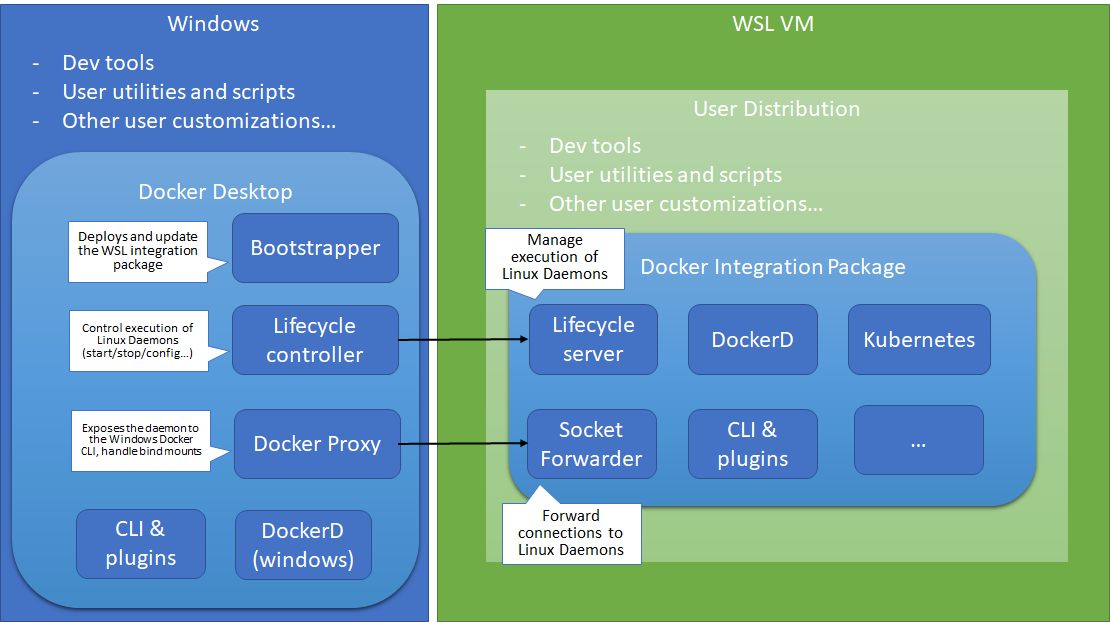
\includegraphics[width=.7\textwidth]{images/docker-in-wsl2.png}
\caption[Visualstudio]{Visualstudio.com redirects to Microsoft's site.{\tiny{Microsoft.com}}} 
\label{figure:docker-in-wsl2}
\end{figure}


\url{https://code.visualstudio.com/blogs/2020/03/02/docker-in-wsl2}

\section{Docker Networking}

Here the ``Network Path'' is considered to be the wire and packets that
lead from the farthest router to where your organization meets the
internet, the nearest router where your PMachine meets your organization,
(the bits inside that router), where the wire enters the PMachine
(this may be none or more RJ11 or wireless points), the IP stack,
the pathway through the kernel, the user-space layer, and the application
layer.

\begin{figure}[h!]
\centering
%%\phantomsection
%%\addcontentsline{toc}{section}{}
%%\caption{} %% \caption{{\tiny{citation}}} 
%%\includepdf[angle=90,width=\textwidth]{}); %% with package pdfpages
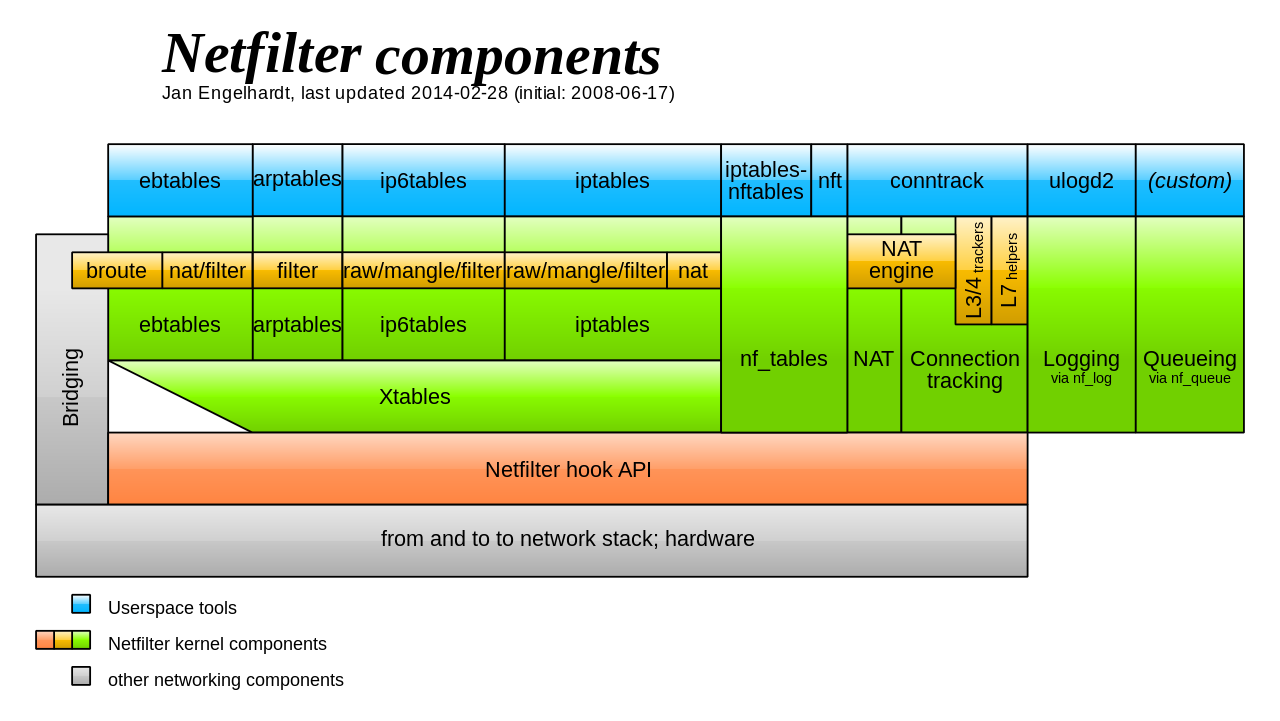
\includegraphics[width=.75\textwidth]{images/1280px-Netfilter-components-svg.png}
\caption[Linux network overview]{Linux network layers in general.\;\;{\tiny{\cite{1280px-Netfilter-components-svg}}}} 
\label{figure:netfilter}
\end{figure}

\clearpage

This builds on the 5-layer TCP/IP model, in that the electro/mechanical way
the signal arrives inside the hardware of the PMachine can be through
some 'interface'\footnote{Run ifconfig or 'ip -addr'.} \index{net-tools vs iproute2}

\begin{table}[h!]
\centering
\begingroup \fontsize{10pt}{10pt}
\selectfont
\begin{tabular}{| l | l |}
\hline
ifconfig command & New ip command   \\
\hline
arp -a                              & ip neigh    \\ 
arp -v                              & ip -s neigh    \\ 
arp -s 192.168.1.1 1:2:3:4:5:6      & ip neigh add 192.168.1.1 lladdr 1:2:3:4:5:6 dev eth1    \\ 
arp -i eth1 -d 192.168.1.1          & ip neigh del 192.168.1.1 dev eth1    \\ 
ifconfig -a                         & ip addr    \\ 
ifconfig eth0 down                  & ip link set eth0 down    \\ 
ifconfig eth0 up                    & ip link set eth0 up    \\ 
ifconfig eth0 192.168.1.1           & ip addr add 192.168.1.1/24 dev eth0    \\ 
ifconfig eth0 netmask 255.255.255.0 & ip addr add 192.168.1.1/24 dev eth0    \\ 
ifconfig eth0 mtu 9000 i            & p link set eth0 mtu 9000    \\ 
ifconfig eth0:0 192.168.1.2         & ip addr add 192.168.1.2/24 dev eth0    \\ 
netstat                             & ss    \\ 
netstat -neopa                      & ss -neopa    \\ 
netstat -g                          & ip maddr    \\ 
route                               & ip route    \\ 
\hline
\end{tabular}
\endgroup
\caption[Net-tools vs IProute2]{A ifconfig vs ip command quick summary.}
\label{table:ifconfigvsipcommand}
\end{table}

\subsection{IPTABLES}

The Docker Container interfaces with the internet via its own
bridge. The container has its own Linux layer with 'cgroups' and
'namespaces'. The Ethernet WAN, passes through iptable filtering
within the main router, any intervening router, the PMachine's
OS, the docker daemon and finally the container's OS. There may
be a few extra layers, policies and general strategies (NAT,SNAT,DNAT,PAT)
that for the rough sea for you app's packets to interoperate with
the app you need at the other end.

There are a few tables:


\definecolor{purple}{rgb}{0.8,0,0.75} % keywords
\lstset{language=bash, basicstyle=\scriptsize,numbers=left,
    numberstyle=\tiny,basicstyle=\small,
    stepnumber=5,numbersep=6pt, showstringspaces=false,breaklines=true
    columns=fixed,basewidth=.57em,
    keywordstyle=\color{purple},
    commentstyle=\color{red}}
\begin{lstlisting}
# as root
echo "# myiptables" > /tmp/myiptables    # start the file
for f in filter nat mangle raw; do
  echo "# table type : $f" >> /tmp/myiptables
  iptables -t $f -L >> /tmp/myiptables
done
\end{lstlisting}

\clearpage
The output:

\begin{tcolorbox}[breakable]
  \begingroup \fontsize{6pt}{6pt}
\selectfont
%%\begin{Verbatim} [commandchars=\\\{\}]
\begin{verbatim} 
# myiptables
# table type :filter
Chain INPUT (policy ACCEPT)
target     prot opt source               destination         

Chain FORWARD (policy DROP)
target     prot opt source               destination         
DOCKER-USER  all  --  anywhere             anywhere            
DOCKER-ISOLATION-STAGE-1  all  --  anywhere             anywhere            
ACCEPT     all  --  anywhere             anywhere             ctstate RELATED,ESTABLISHED
DOCKER     all  --  anywhere             anywhere            
ACCEPT     all  --  anywhere             anywhere            
ACCEPT     all  --  anywhere             anywhere            

Chain OUTPUT (policy ACCEPT)
target     prot opt source               destination         

Chain DOCKER (1 references)
target     prot opt source               destination         
ACCEPT     tcp  --  anywhere             172.17.0.4           tcp dpt:postgresql
ACCEPT     tcp  --  anywhere             172.17.0.3           tcp dpt:postgresql

Chain DOCKER-ISOLATION-STAGE-1 (1 references)
target     prot opt source               destination         
DOCKER-ISOLATION-STAGE-2  all  --  anywhere             anywhere            
RETURN     all  --  anywhere             anywhere            

Chain DOCKER-ISOLATION-STAGE-2 (1 references)
target     prot opt source               destination         
DROP       all  --  anywhere             anywhere            
RETURN     all  --  anywhere             anywhere            

Chain DOCKER-USER (1 references)
target     prot opt source               destination         
RETURN     all  --  anywhere             anywhere            
# table type :nat
Chain PREROUTING (policy ACCEPT)
target     prot opt source               destination         
DOCKER     all  --  anywhere             anywhere             ADDRTYPE match dst-type LOCAL

Chain INPUT (policy ACCEPT)
target     prot opt source               destination         

Chain OUTPUT (policy ACCEPT)
target     prot opt source               destination         
DOCKER     all  --  anywhere            !localhost/8          ADDRTYPE match dst-type LOCAL

Chain POSTROUTING (policy ACCEPT)
target     prot opt source               destination         
MASQUERADE  all  --  172.17.0.0/16        anywhere            
MASQUERADE  tcp  --  172.17.0.4           172.17.0.4           tcp dpt:postgresql
MASQUERADE  tcp  --  172.17.0.3           172.17.0.3           tcp dpt:postgresql

Chain DOCKER (2 references)
target     prot opt source               destination         
RETURN     all  --  anywhere             anywhere            
DNAT       tcp  --  anywhere             anywhere             tcp dpt:55432 to:172.17.0.4:5432
DNAT       tcp  --  anywhere             anywhere             tcp dpt:55435 to:172.17.0.3:5432
# table type :mangle
Chain PREROUTING (policy ACCEPT)
target     prot opt source               destination         

Chain INPUT (policy ACCEPT)
target     prot opt source               destination         

Chain FORWARD (policy ACCEPT)
target     prot opt source               destination         

Chain OUTPUT (policy ACCEPT)
target     prot opt source               destination         

Chain POSTROUTING (policy ACCEPT)
target     prot opt source               destination         
# table type :raw
Chain PREROUTING (policy ACCEPT)
target     prot opt source               destination         

Chain OUTPUT (policy ACCEPT)
target     prot opt source               destination         
\end{verbatim}
\endgroup
%% \end{Verbatim}
\end{tcolorbox}


In General IP Tables enter the picture.

\url{https://www.cyberciti.biz/tips/linux-iptables-examples.html}

Has a decent description of commands etc.

Change commands require root privileges This includes query commands
and commands that cause changes.  Use \dhl{sudo} for each command, or
\dhl{sudo -s} (dangerous way) and have at it.

In particular the

\begin{tcolorbox}[breakable]
\begingroup \fontsize{10pt}{10pt}
\selectfont
%%\begin{Verbatim} [commandchars=\\\{\}]
\begin{verbatim} 
iptables -L --line-numbers   # See the rules with numbers
iptables -D INPUT 3          # Find the particular one, -D delete it from IMPUT side.
\end{verbatim}
\endgroup
%% \end{Verbatim}
\end{tcolorbox}



\section{Cleaning House}

This little ditty removes ALL the images.


\verb=sudo docker rmi $(sudo docker images -aq) --force=



\section{IRAF/PyRAF Multiverse}

\begin{figure}[h!]
\centering
%%\phantomsection
%%\addcontentsline{toc}{section}{}
%%\caption{} %% \caption{{\tiny{citation}}} 
%%\includepdf[angle=90,width=\textwidth]{}); %% with package pdfpages
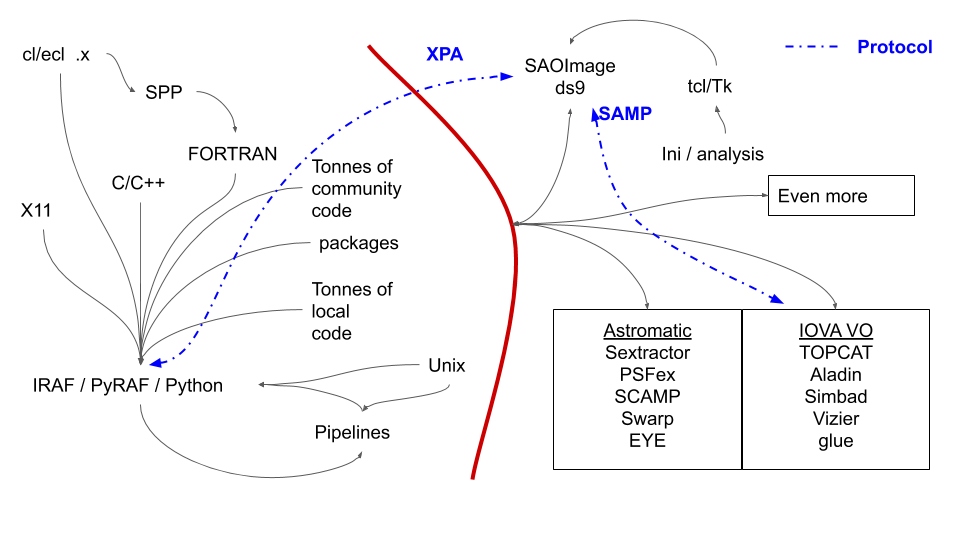
\includegraphics[width=\textwidth]{images/IRAFUniverse.png}
\caption[IRAF/PyRAF Multiverse]{IRAF/PyRAF Multiverse of players.} %% \caption{{\tiny{citation}}} 
\label{figure:Multiverse}
\end{figure}
\clearpage

IRAF\cite{1984BAAS...16..497V}~\footnote{IRAF (Image Reduction (and)
  Analysis Facility)}, eventually grew into 'cl' or command
language. IRAF is a 'collection' of routines, from various authors at
various institutions, designed to work with the institutions data.
Eventually, the community settled on NOAO coordinating both IRAF, its
language mechanisms and distribution; and the rough agreement for
image transfer using FITS\cite{FITSStandard-1} (Flexible Image
Transport System).Remember, the first word is ``Flexible''.

Its complicated: See Figure \ref{figure:Multiverse}.

IRAF's basic scripting language (\dhl{cl}) was quickly extended into
the modern \dhl{ecl} (extended-cl). Rather than an ``eecl'', Python's
readline command line interpreter
\cite{PyrafProgrammersGuide,CLProgrammersGuide}) was adapted to create
PyRAF\cite{2006hstc.conf..437G} -- to support most existing ecl
'tasks' together with their module subroutine equivalents. However,
copyrighted algorithms and a heavy dependency on early X11 has IRAF
'wedged' \endnote{\textbf{\emph{wedged adj.}}
  \index{IRAF!\textbf{\emph{def}}.}

1. To be stuck, incapable of proceeding without help. This is
different from having crashed. If the system has crashed, it has
become totally non-functioning. If the system is wedged, it is trying
to do something but cannot make progress; it may be capable of doing a
few things, but not be fully operational. For example, a process may
become wedged if it deadlocks with another (but not all instances of
wedging are deadlocks). See also gronk, locked up, hosed, hung (wedged
is more severe than hung). 2. Often refers to humans suffering
misconceptions. "He's totally wedged -- he's convinced that he can
levitate through meditation." 3. [Unix] Specifically used to describe
the state of a TTY left in a losing state by abort of a
screen-oriented program or one that has messed with the line
discipline in some obscure way.

There is some dispute over the origin of this term. It is usually
thought to derive from a common description of recto-cranial
inversion; however, it may actually have originated with older
`hot-press' printing technology in which physical type elements were
locked into type frames with wedges driven in by mallets. Once this
had been done, no changes in the typesetting for that page could be
made.

For this and more jargon: https://www.eps.mcgill.ca/jargon/jargon.\#wedged
}.

While PyRAF/IRAF has greatly reduced its dependency on i386 libraries,
it still heavily depends on early X-Windows code\footnote{X has
  essentially been frozen at X11 since 1986. The font generation is
  downright primitive.}. Ubuntu, a popular Linux operating system, is
dropping 32-bit (i386) program support with the release of 19.04
(2019).  The X11 replacement ``Wayland'' \index{Wayland} and other
attempts to replace X11 have met with limited successes. X11 support was
phased out of the Apple OSs since the 2012 framework and has relied on
external packages like XQuartz etc.  PyRAF/IRAF has resolved
licensing issues from use of algorithms from ``Numerical Recipes for
C'' \cite{PresTeukVettFlan92} - a popular academic reference in the
day. \index{X11!introduction}

PyRAF/IRAF is under pressure from the younger astronomers putting a
heavy reliance of Python, Astropy, and very modern computing
environments. This is slow-going as the inspired receive their PhDs
and their efforts wane in the face of new duties. \index{Astropy!introduction}

This adds up to the fact that a very large user base (by astronomy
scales) is losing the ability to perform analysis and/or suffer from a
daunting learning AND development curve!

These notes explore bridging the PyRAF/IRAF and Astropy communities.
This article focuses on moving into a Ubuntu 18.04+ OS image within a
Docker Container that will be available on Linux/Mac/Win10 platforms.

The one other issue to put into people's brains is Anaconda's reliance
on the Intel Math Kernel Library for Numpy is broken on AMD processors.
\index{numpy!Math Kernel Library} \index{numpy!AMD}

Carl Boettiger \cite{DBLP:journals/corr/Boettiger14} makes a good
argument for disseminating scientific projects in a 'ready to run'
docker based environment.


\section{AAVSO}

Enter star name; browser, save the image; use photometry like
cut/paste: the paste is more of a tsv but with issues:

\vspace{-.15cm}
\begin{enumerate}\addtolength{\itemsep}{-0.5\baselineskip}
   \item   Lable is 'Chart ID'
   \item   There is no link to get a decent TSV/CSV/XLS.
   \item   There are embedded UNICODE eyecandy characters.
   \item   Some columns have two fields! STUPID.
\vspace{-.15cm}
\begin{enumerate}\addtolength{\itemsep}{-0.5\baselineskip}
   \item     RA and DEC
   \item     V has goofy mag statement X.XXX (X.XXX)XX 3 fields?
   \item     B-V is a DELTA with (X.XXX)
\end{enumerate}

   \item   000-BKP-763 is cited with missing mag error, where B-V    has an error. 
   \item   000-BKP-763 has missing mag error as a unicode 0x2014.
   \item      Recommend nan, can not error-propagate nan.
   \item   Make a data dictionary/algorithm dictionary. 
\end{enumerate}



Recommend
$RA/DEC$ be $RA_ICRS/DEC_ICRS$ and be in degrees no decorator
   (put the decorator as [deg] in header
$RA_2000/DEC_2000$ be in sexigesimal hours
Magnitudes be split into 2 or 3 columns
Footnote to table explaining fields.
Make fields machine parsable with python snippets to parse.

\section{Planning}

\begingroup \fontsize{10pt}{10pt}
\selectfont
%%\begin{Verbatim} [commandchars=\\\{\}]
\begin{verbatim} 
Observations
  usw
     targets
        targetname
          <stuff>
\end{verbatim}
\endgroup
%% \end{Verbatim}

\subsection{ds9}


General:
   Set the font sizes: Default is 10, may want 12
   Bllank/inf/nan to yellow (actually get a chance to see one)
Startup:
   Initialize XPA and offer SAMP connection (Tie to TOPCAT and Aladin)

Menus and Buttons : See below.

Magnifier: 8x or 16x really zoom into a 'star'

Edit \menu preferences.

Graphs: Axis linear; Method Average/sum
Annulus! 

Analysis log>?

Pixel Table: 13   (bigger is better)
Catalogs : Color Cyan

Postscript: DPI 600 (for publication)

\subsubsection{Menus and Buttons}

Here certain preferences are set.
Very Important: first off, use retions and projection.
This makes the projection tool the default one.

You can adjust what is ticked as default in the menus
and what appears in the button bar.
For example: wake up in vertical mode.

\subsubsection{Finder Charts}

Load the image.
Under Analysis \menu coordinate and coordinate grid:

In the menu; you may save the file.
Save this to the general usw dir for the instrument.


\begingroup \fontsize{10pt}{10pt}
\selectfont
%%\begin{Verbatim} [commandchars=\\\{\}]
\begin{verbatim} 
Type
Publication
Exterior Axes
Exterior Numerics

Coordinate
WCS
ICRS
degrees or (Sexigesimal) 

Grid
Color Black (or White)
Line (thickness or dash)

Axes
Color Black

Numerics
Color black
Font (size)

Labels
Color
Font

Tickmakrs
Color
Line (size)

Border (It sometimes wraps!)
Color Black
Line (2 a tad thicker)

Labels:
Axis 1 RA (IRCS [deg]) uncheck the box
Axis 2 Dec (IRCS [deg]) uncheck the box

Spacing:
Title   12
Axis 1   0
Axis 2   5
\end{verbatim}
\endgroup
%% \end{Verbatim}





\subsubsection{Hacking ds9}

Only to say, you can add your own tcl to ds9.ini. That is very powerful.



\begingroup \fontsize{10pt}{10pt}
\selectfont
\begin{Verbatim} [commandchars=\\\{\}]
Analysis\menu
  Survey\menu POSS2/UKSTU (or other red) 
  Use 45 arcmin as the FOV
  Save file <target>_DSS_Finder
Analysis\menu Catalogs\menu Database \menu SIMBAD
Catalog Tool: \menu Symbol Color \menu Cyan
Catalog Tool: \menu Symbol Advanced
   Text $FLUX_B
\end{Verbatim}
\endgroup

\section{Handy Docker Phrases}

\begingroup \fontsize{10pt}{10pt}
\selectfont
%%\begin{Verbatim} [commandchars=\\\{\}]
\begin{verbatim} 
docker run -it --hostname myfoo # override the default ID as hostname.
\end{verbatim}
\endgroup
%% \end{Verbatim}

%%% ADDAPPENDIX


%% use a bibitem approach to the references publications etc.
%% (wg-bibitem)



%%\clearpage
\addcontentsline{toc}{section}{References}
\renewcommand*{\refname}{Bibliography and References}
\bibliographystyle{plain}	% bibliographystyle{apalike} and \usepackage{natbib}
\bibliography{BanzaiPipeline}	% expects file "MasterBib.bib"


% https://arxiv.org/pdf/1410.0846.pdf


%%\begin{thebibliography}{80}
%%\usepackage{natbib}   %% bibitems
%%\end{thebibliography}

% /home/git/pre/DaintyDittys.pre/doc/DaintyDittys.tex

%% (wg-texdoc-endnotes)

%%%%%%%%%%%%%%%%%%%%%%%%%%%%%%%%%%%%%%%%%%%%%%%%%%%%%%%%%%%%%%%%%%%%%%%%%%%%%
% Support for endnotes
\begingroup
\renewcommand{\notesname}{\textcolor{red} {Action Items/EndNotes:}}
\parindent 0pt
\parskip 2ex
\phantomsection
\addcontentsline{toc}{section}{\textcolor{red} {Action Items:}}
\def\enotesize{\normalsize}
\theendnotes
\endgroup

\clearpage
\addcontentsline{toc}{section}{Index}
\printindex %% www.cs.usask.ca/resources/tutorials/latex/notes/toc-index.pdf


\end{document}
%%% ENDDOC

http://www.renhuanheng.com/2019/10/10/linux-forward-display-launching-gui-app-from-docker.html

FROM iraf:v1

ENV HOME /home/bob
USER bob

CMD /usr/bin/firefox

/home/git/pre/DaintyDittys.pre/doc/DaintyDittys.tex

docker run -it \
--user 1000:1000 \
--workdir /home/bob \
 -v /tmp/.X11-unix:/tmp/.X11-unix \
 -e DISPLAY=$DISPLAY \
 -h $HOSTNAME \
 -v $HOME/.Xauthority:/home/bob/.Xauthority \
-v $HOME/Astro:/home/bob/Astro \
-v $HOME/iraf:/home/bob/iraf \
 iraf:v2


# wake up as root
docker run -it \
 -v /tmp/.X11-unix:/tmp/.X11-unix \
 -e DISPLAY=$DISPLAY \
 -h $HOSTNAME \
 -v $HOME/.Xauthority:/home/bob/.Xauthority \
-v $HOME/Astro:/home/bob/Astro \
-v $HOME/iraf:/home/bob/iraf \
 iraf:v2

docker run -it \
 -v /tmp/.X11-unix:/tmp/.X11-unix \
 -e DISPLAY=192.168.0.216:$DISPLAY \
 -h $HOSTNAME \
 -v $HOME/.Xauthority:/home/bob/.Xauthority \
-v $HOME/Astro:/home/bob/Astro \
iraf:1.0


---
2020-04-07T21:09:40-0600

Built the docker iraf:v1.0 (should have been 0.95!)
The first stab, blocked on the question in the XOrg load.
Thought I had that one solved.

So...

docker run -it iraf:v1.0

apt-get install -y xorg  # add in the X11 stuff. Has question


%
 Parent
 
 ---
 2020-04-08T11:47:08-0600

docker run -it continuumio/cuupdated -v /home/wayne/play/bob/ir1:/opt/conda/pkgs 
docker cp b76b0dff7ed8:/opt/conda/pkgs .  # get the contents of the clean container

conda config --add channels http://ssb.stsci.edu/astroconda
conda create -n iraf27 iraf-all pyraf-all stsci


---
2020-04-08T22:40:02-0600

docker run

apt-get install -y x11-utils
apt-get install -y x11-apps






%%% ENDDOC tag to move over this tail end stuff

2020-04-10T10:54:00-0600
Handy awk biased to network ss.
\lstset{language=Awk, basicstyle=\scriptsize,numbers=left,
    numberstyle=\tiny,basicstyle=\small,
    stepnumber=5,numbersep=6pt, showstringspaces=false,breaklines=true
    columns=fixed,basewidth=.57em,
    keywordstyle=\color{purple},
    commentstyle=\color{red}}
\begin{lstlisting}
BEGIN {print "hello";}
/.*/ {foo[$5]++; }
END {
for (f in foo) { 
   printf("%s %s\n",f,foo[f]);
}
}
\end{lstlisting}

NAT SNAT DNAT PAT and Port Forwarding
https://www.youtube.com/watch?v=wg8Hosr20yw


wedged adj.

1. To be stuck, incapable of proceeding without help. This is
different from having crashed. If the system has crashed, it has
become totally non-functioning. If the system is wedged, it is trying
to do something but cannot make progress; it may be capable of doing a
few things, but not be fully operational. For example, a process may
become wedged if it deadlocks with another (but not all instances of
wedging are deadlocks). See also gronk, locked up, hosed, hung (wedged
is more severe than hung). 2. Often refers to humans suffering
misconceptions. "He's totally wedged -- he's convinced that he can
levitate through meditation." 3. [Unix] Specifically used to describe
the state of a TTY left in a losing state by abort of a
screen-oriented program or one that has messed with the line
discipline in some obscure way.

There is some dispute over the origin of this term. It is usually
thought to derive from a common description of recto-cranial
inversion; however, it may actually have originated with older
`hot-press' printing technology in which physical type elements were
locked into type frames with wedges driven in by mallets. Once this
had been done, no changes in the typesetting for that page could be
made.

\url{https://www.eps.mcgill.ca/jargon/jargon.html#wedged}


2020-04-16T11:38:01-0600

apt-get download packages...
cd /var/cache/apt/archives
scp *deb wayne@192.168.0.216:/home/git/pre/astromatic.pre/docker/offline/cache

In the container:
cd /var/cache/apt/archives

/home/git/pre/astromatic.pre/docker/offline/cache/docker/ubuntu

\dirtree{%
.1 Observations.
.2 \dhl{/ddMMMyyyy/}  \# \dhl{local dates data}.
.3 usw                \# \dhl{Nights collection}.
.4 reduce.cl          \# \dhl{template}.
.4 reduce.pyraf       \# \dhl{template}.
.3 RawData            \# \dhl{Nights Raw Data}.
.3 PreAnalysis         \# \dhl{The basic work}.
.3 Analysis            \# \dhl{Non-pipeline work for pre-publication}.
.2 usw \# \dhl{Global templates etc}.
.3 Targets \# \dhl{Global target collection usws}.
.4 \dhl{<target>}.
.5 hints.ans.
.5 cfg.ans.
.5 target.tsv.
.5 finder.png.
.5 Catalog\_AAVSO.tsv.
.5 Catalog\_UCAC4.tsv.
.5 Catalog\_REFCAT2.tsv.
}
